\chapter{Fundamentação Teórica}
\label{cap:fundamentacao-teorica}

	De acordo com Oliveira e ANDRADE (2010), Sistemas embarcados são sistemas computacionais completos e independentes que possui a parte física (Hardware) e Lógica (Software ou Firmware), mais simples que um computador de propósito geral (Desktops), encarregados de executar apenas uma função determinada - tarefas pré-determinadas, com requisitos específicos, na qual executam geralmente repetidas vezes. Por serem muito simples, muitas vezes esses sistemas não têm flexibilidade (de software e de hardware) que lhes permita fazer outras tarefas quaisquer que não sejam aquelas para as quais foram desenhados e desenvolvidos.
Um grande responsável pela expansão do uso e aplicação dos sistemas embarcados foi a utilização do microcontrolador, pelo seu baixo custo, versatilidade e tamanho reduzido. Muitos microcontroladores podem ser conectados a dispositivos analógicos, permitindo o uso de sensores diversos. Isso permite a criação de dispositivos simples, que monitoram temperatura, umidade, entre outros fatores, executando ações predefinidas em caso de mudanças.
Em geral os sistemas embarcados possuem uma capacidade de processamento reduzida em comparação com computadores desktops. Ao invés de utilizar microprocessadores, os desenvolvedores preferem utilizar microcontroladores, pois estes já possuem diversos periféricos integrados no mesmo chip.V850, FR-V Outra diferença é a variedade de arquiteturas disponíveis tais como ARM, MIPS, Coldfire/68k, PowerPC, x86, PIC, 8051, Atmel AVR, Renesas H8, SH, M32R, Z80 e Z8.
Os sistemas embarcados comunicam-se com o meio externo através de periféricos. Estes periféricos podem ser combinados com o processador (como no caso dos sistemas microcontrolados) ou associados no sistema.
Entre os periféricos mais comum temos:
	Entrada de dados através de teclas (geralmente através de teclados feitos com varredura matricial)
Leds
	Displays de LCD (sendo os mais comuns os alfanuméricos por exemplo o HD44780)
Interface serial - (Por exemplo RS 232, I2C)
Universal Serial Bus - (USB)
TCP/IP

Hardware 
Graças a tecnologia baseada em transistores é possível miniaturizar componentes como os circuitos integrados, processadores e seus periféricos com baixo custo através de encapsulamento permitiu ter uma variedade de dispositivos para uma determinada aplicações e aperfeiçoa-la assim como os conversores analógico- digital (AD) capaz de digitalizar toda a informação em apenas uma fração de tempo.  Possui na sua arquitetura: Unidade Central de Processamento composto por unidade Logica e aritmética, Unidade de controle, Sistema de memória composto por memória de acesso aleatório e de Armazenamento e Sistemas de Entrada e saída interligados por meios de barramentos.
Firmware
É um tipo de Software Embarcado que controla o Hardware usando linguagens de baixo nível (Linguagem de máquina). Ele possui os principais componentes: Sistema básico de entrada e saída (BIOS) BASIC IMPUT OUTPUT SYSTEM serve parar inicializar o sistema, checar os dispositivos e carregar o Sistema Operacional (SO); SETUP responsável por alterar os parâmetros da memória de configuração (CMOS) que é usada para gravar as configurações do SETUP em uma pequena área de memória volátil alimentado por uma bateria. Podendo operar em tempo real onde determinadas tarefas tem o seu prazo compatíveis com a ocorrência dos eventos.
Controller Area Network (CAN)
Baseada em aplicações em tempo real um meio para transmissões de redes e controla o fluxo e propagação de mensagens sendo necessario um cotrole rígido de erro para que haja eficácia no recebimento de mensagens.
Godoy et al; 2010. Afirma que O CAN (Bosch, 2006) é um protocolo de comunicação digital serial e não determinístico, onde a comunicação de dados é baseada em mensagens formadas por quadros de bits com determinada função. Entre esses quadros de bits, existe o campo identificador (identifier ID) que caracteriza e define a prioridade de cada mensagem. O valor do identificador de uma mensagem em uma rede CAN é exclusivo e quanto mais baixo seu valor, maior será a prioridade da mensagem. Os sinais elétricos digitais do CAN são representados pelo nível recessivo (nível lógico 1) e nível dominante (nível lógico 0), sendo eles sinais diferenciais entre os dois fios da rede.(GODOY et al; 2010)



\acrlong{ARM},\acrlong{MIPS},\acrlong{PIC},\acrlong{AVR},\acrlong{LCD},\acrlong{USB},\acrlong{TCP},\acrlong{IP},\acrlong{AD},\acrlong{BIOS}


	
	\begin{figure}[h!]
		\centering
		\Caption{\label{fig:exemplo-2} Diagrama básico de um sistema embarcado dotado de um microcontrolador monitorando o ambiente.}	
		\UNIFORfig{}{
			\fbox{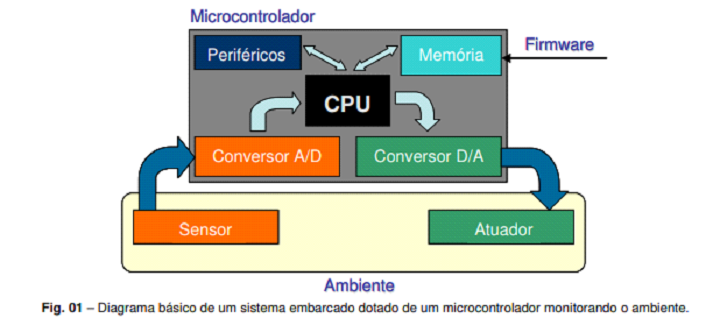
\includegraphics[width=14cm]{figuras/fig01}}
		}{
			\Fonte{Elaborado pelo autor}
		}
		
	\end{figure}
	
		\begin{figure}[h!]
		\centering
		\Caption{\label{fig:exemplo-3} Logica de um sistema embarcado usando um microprocessador como unidade de processamento.}	
		\UNIFORfig{}{
			\fbox{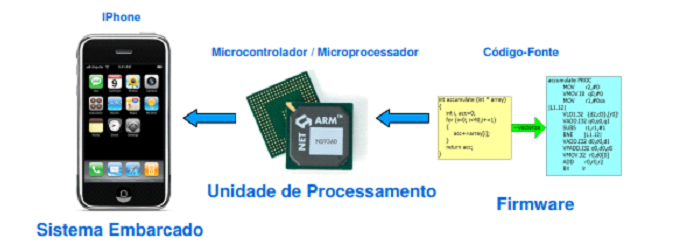
\includegraphics[width=14cm]{figuras/fig02}}
		}{
			\Fonte{Elaborado pelo autor}
		}	
	\end{figure}
	




